\documentclass{ltjsbook}
\usepackage{docmute} 
\usepackage{../../myStyle} 

\begin{document}
\chapter{心理統計を始める前に}
\label{ch01_introduction}
これから「心理統計学」を学んでいくわけですが，皆さんはそもそも心理学と統計学が深く関わっていることをイメージしていたでしょうか。もし心理学なのに数学の話があるの？ 心理学と統計になんの関係があるの？ と思った人は，そもそも心理学というのはどういうものをイメージしていたでしょうか。

第1回ではまず，心理学を学ぶにあたってなぜ統計学が必要なのかを考えます。そのためには，心理学が科学(Science)であることを知る必要があります。科学であるとはどういうことかを理解し，そのために数量的表現が有用であることをしっかりと理解してもらわなければなりません。

%%%
\section{はじめに}

みなさん，心理統計の世界，いいえ心理学の世界へようこそいらっしゃいました。

みなさんは心理学という言葉を，はじめて聞いたのはいつだったのか覚えていないのではないでしょうか。それぐらい一般的に使われていますが，さてそこではどのようなことを研究しているのか，皆さんはどんなイメージをお持ちでしょうか。皆さんが何をきっかけで心理学を志したのかによって，それは随分と異なってくると思います。

ある人はテレビドラマ「逃げるは恥だが役に立つ」をみて，主人公の女性が心理学の大学院をでたことから興味を持ったのかもしれません。あるいはスクールカウンセラーが学校にいたから，なんなら少し相談に乗ってもらったから，心理職というのがどのようなものなのか興味を持ったのかもしれません。

あるいはまた，テレビドラマ「科捜研の女」をみて，主人公が働く科学捜査研究所における心理職を知ったのかもしれません\footnote{科捜研には物理，化学，法医，文書，心理の5職種があり，文書鑑定(筆跡鑑定)と心理(ポリグラフ検査)を一人の技師が兼ねているところもあります。}。実際の科捜研における心理職は虚偽検出を行っており，これには(生理)心理学の知見が生かされています。

他にも高校までの科目として，倫理や現代社会でフロイド，エビングハウス，マズローなどの名前を聞いた人もいるかもしれません。知らなくても今から学ぶので問題ないのですが，それでもフロイドとポリグラフ検査はどう繋がるんだろう，と首を傾げるひともいるでしょう。心理学の知見は他にも，進路相談・職業指導や，街中に溢れるいろいろな工業製品のデザイン，トリックアートから神経生理学，果てはAI(人工知能)などにも関わってきます。

たとえば法学部では法律の勉強をするだろうということはわかりますが，「心理学を学んでいるよ」と誰かに言ってみても「それは何をするの？ 」と聞かれ，「心が読めるのか」とからかわれることもあるかもしれません。\textcite{Michimata200903}には，次のような一節があります。

\begin{quote}
	心理学を「盛岡名物わんこそば」だとしよう。わんこそばはうまいし，おもしろいし，実に素晴らしいものだ。しかし，十分な知識のない人が，わんこそばについて勝手に空想的なイメージ(かわいいちいさなお椀にはいったおいしいおそばなど)を形成して，何の心構えもなく実際のわんこそばを注文したらどうなるだろうか。それはきっとかなり恐ろしい体験に違いない。
\end{quote}

皆さんはまるでこの人のように，こんなものが心理学だったのかと驚かれるのではないかと思います。心理学は\textbf{名前は知られているが中身を知られていない学問}なのです。心理学が自分のイメージと違うなと思った人，とくにイメージはなかった人，色々いると思いますが，皆さんが今持っているイメージはこの4年間ですっかり変わってしまうと思います。少なくとも最初のメッセージとして，ともかく色々な領域に触れて自分のイメージが変わることを恐れないでください，ということを伝えておきたいと思います。(心理)統計なんて嫌だよ，と思ったひとも，いったん真っ白な気持ちで受講してくれれば嬉しく思います。

\section{心理学とはどういう学問か}

ところで「しんりがく」という言葉はどこで区切るかご存知ですか？ 「し/んりがく」?「しん/りがく」?「しんり/がく」?

正解は「しん/りがく」です。心の理学，つまり「こころの\ruby{理}{ことわり}」についての学が心理学なのです。
さらにいうと，「学」ですから，エンターテインメントや怪しげな術ではなく，知識の体系であるというのが大前提です。
そして知識の体系とは，「積み重ねることができるもの」であり「誰にでも共有できるもの」でなければなりません。
だからこそ大学で教育できるのです。
逆に考えてみるとよくわかります。
積み重ねられず，天啓を受けて，あるいは生まれ持った特殊な技能で達成できるものは学問ではありません。また，誰にも言えない特別な秘伝により限られた人や集団にしか教えられない情報も，宗教や奇跡，マジックや詐欺の領域に属するからです。
心理学に神秘的で言葉にできない特殊な何かを求めている人には，残念ですがそれは心理学ではない，とお伝えしなければなりません\footnote{「なんだよー，さっきいろいろな心理学があるって言ったじゃないかよー。本当はこっそり秘伝の術があるんだろう，カウンセリングとか催眠術とかさあ。」と思っている人もいるかもしれませんが，残念ながらそれは心理学どころかそもそも学問じゃないんです。世の中には超心理学だとか，サイコなんとかだとかメンタルなんとかだといって，商売ネタに``心理''というワードを使う輩が後を絶たないから，心理学の誤解は無くならないんですよねえ。}\footnote{余談ですが，大学での学問はすべてこうした「秘伝」を否定するものです。もし言語的に伝えられない合理的でないものがあるならば，それは大学で取り扱うものではありません。もし皆さんが学びたいと思っているのに，合理的な理由なく大学教員が教えてあげないというならば，アカデミックハラスメントに該当します。}。

すでに述べたように，心理学は幅広い領域をカバーしています。それでも大きく分けると2つの分類ができるでしょう。\textcite{Shimoyama2001}は次の表\ref{tbl:01_01}のように分類しています。

\begin{table}[hb]
	\centering
	\caption{\textcite{Shimoyama2001}による心理学の分類}
	\begin{tabular}{ccc}
		アプローチ   & 実証主義的アプローチ    & 了解的アプローチ       \\\hline
		主な分野    & 基礎心理学         & 臨床心理学          \\
		手法      & 自然科学的手法       & 臨床的手法          \\
		対象となる側面 & 客観的事実         & 主観的事実          \\
		データ収集   & 実験・調査         & 臨床実践           \\
		データの特徴  & 量的データ(客観的データ) & 質的データ(物語性)     \\
		モデルの有効性 & 理論的な検証可能性     & 現実状況を理解する際の有効性 \\
		対象者との関係 & 介入しない         & 積極的な関与(関与観察)   \\\hline
	\end{tabular}
	\label{tbl:01_01}
\end{table}
ここでは心理学のアプローチを，実証主義的なアプローチと了解的なアプローチに二分しています。一般的には基礎と応用といった名称で呼ばれることもありますが，内容的にはこちらの区分の方が良いでしょう。主な分野としてそれぞれ基礎心理学，臨床心理学が挙げられていますが，基礎心理学のなかには知覚，生理，学習，認知といったさらに細かい学術領域があります。

2つのアプローチが大きく異なるのは，続く研究の方法論的箇所です。実証主義的アプローチは自然科学的手法を模範とし，客観的事実に基づく実験や調査を行い，理論的な検証・予測を目的とします。一方で了解的アプローチの目的は第一に，クライアントの状態が良くなるところにあり，対象に積極的な関与をしますし，理論よりも現実状況を理解する有効性を目的とするのです。とはいえいずれにも共通するのは，これが科学(Science)であり，データに基づく知識の積み重ねであるという点です。

いずれにせよ，心理学者は心を読んだり，操ったりしているわけではありません。心というものがあるとしたら，どういう機序(＝メカニズム，仕組み，因果関係)があるかを明らかにしようとしているのです。実は，心というものがあるのか，ないのか，それもわかりません。目にも見えず触ることもできないのですから。あなたの隣にいる人だってよくできたロボットかもしれないですよ？ \footnote{「スワンプマン」と呼ばれる思考実験の例があります。興味があれば「スワンプマン」で調べてみてください。}そしてこの，対象が客観的・物理的に把握できない，社会的実在や主観的経験であることが心理学の難しさなのです。

心理学は「目に見えない対象を研究する」という難しい課題にチャレンジし続けている学問です。それでいて物理学(物質の理の学)のように，規則性，法則性を探そうとしている学問です。気を付けないと，超魔術やスピリチュアル，宗教のようなものになってしまいます。心理学は，「知識の体系」＝「学」＝科学(Science)であることを忘れないで欲しいのです。

\section{近代科学の特徴}

さて心理学が科学であるというならば，そもそもその科学とはなんでしょうか。西洋の歴史を考えてみると，そもそもギリシア哲学から学問が発生し，その後は中世に至るまでキリスト教が「世界を説明する教義」として支配的な考え方を提供していました。これが近代科学になるためには，ニュートンやガリレオなどによるルネサンスを待たねばなりません。そこでは一体どういう考え方の転換があったのでしょうか？

近代科学の特徴は，次の4つにまとめることができるでしょう。また，それぞれの考え方に関係した人の名前を挙げています。
\begin{itemize}
	\item 実験主義：ティコ・ブラーエやケプラーによる天文記録，ガリレオのさまざまな実験
	\item 数量主義(\keytermL{数学的現象主義}{すうがくてきげんしょうしゅぎ})：ガリレオやニュートンによる記述
	\item 機械論的発想：デカルトや，マクスウェルのデモンに代表される考え方
	\item 要素還元主義的：デカルトの「第二の格率」，「分割と統合」といった考え方
\end{itemize}

まず実験主義である，というのは「教科書に書いてあるから確かめなくてもいいでしょ」という考え方への反発です。「本当かどうか，確かめてみようじゃないか」というスタイルです。西洋では長らく聖書に書いてあることが世界の答えでした。聖書には重たいものが軽いものよりも先に落ちる，と書いてありました。だって神様がそうしてくれたのだから，というわけです。このことを疑うのは，神を疑うことであり，そんな人は地獄に落ちるぞ，と言われたりします。

しかしこれを確かめてみよう，と実験したのがガリレオです。ピサの斜塔から重たいものと軽いものを同時に落とし，同時に着地することを確認する。実際にやって確かめなければならない，思弁的に論じているだけではダメだ，というわけです。

他にも，ティコ・ブラーエやケプラーといった天文学者は天体の動きを何年にもわたって記録し，どういう法則性があるのかを考えていました。これも実際にデータをとって考えてみるという意味では実験主義的な態度であり，これが科学の基本的なスタイルなのです。

数量主義あるいは数学的現象主義は，数学で現象を記述しようという考え方です。ニュートンは重力を発見した，と言われますが，正確には力がどのように働くのかを数式で表現したのであり，重力を見たわけではありませんよね。データをとってその関係性を記述することで，世界の理解を深めようと考えているのです\footnote{神様の存在を疑ったり反抗したりするのではなく，逆に「こんなにも完璧に自然を設計している神様まじパネエ」という信仰心から研究が重ねられていたようです。詳しくは\textcite{IkeuchiR2014}や\textcite{Hebizo2016}などがおすすめです。}。大事なポイントは，重力が何か(What)ではなく，どのように働くか(How)，という問いの大転換をしたことであり，これが近代科学の基礎を築いたのです。

機械論的発想というのは，「世界は機械＝メカだ。メカニズム(機序)があるんだ」という考え方です。西洋では長らく，世界は神様が作ったものだから，その仕組みを探ったりしたらバチが当たる，と考えられていました。デカルトは「神様が作ったのは「心」で，肉体とかの「体」はいくらでも分解して調べて，神様の考えを勉強させてもらったらええんやで」と考えました\footnote{関西弁は著者の意訳によるものです。}。
このメカニズムを探ろう！というのが科学の目的であるということです。

最後に要素還元主義的であるというのは，「要素」に戻していこう，という考え方です。大きな問題を小さな要素に分解していき，確実にわかることを積み重ねていけば，いつかは大きな問題全体がわかる，という考え方です。これもデカルトの考え方で，「方法序説」という本に書いてあるので興味があれば読んでみてください\parencite{Descartes}。大問題を小問題に分割していこう，というのも近代科学的アプローチの基本です。

さて，心理学は科学ですから，ここにあげた4つの基本的な姿勢はそのまま継承しています。また，この4つの特徴の根本にあるのは\keytermL{私秘性の排除}{しひせいのはいじょ}にあるということにも注意してください。
私秘性とは聞き慣れない言葉かもしれませんが，要するに「私だけが知っている秘密」という性質であり，これを徹底的に排除しようとするのが科学的な姿勢なのです。
私，というのは一個人はもちろん，教会といった特定の組織，ひいては全知全能の神様すら含まれるでしょう。
説明できないところなくし，徹底的に言語化すること，誰にでもわかるように世界を説明することが，科学の究極的な目的なのです\footnote{科学というのはそういう意味で，本質的にコミュニケーションなのです。}。

ですから心理学も当然，「実験的」で「数量的」で「機械論的」で「要素還元主義的」なアプローチをとります。問題を細分化しつつ，実際に実験や介入を経て，その機序を明らかにしていくわけです。でもここで，なんで数字を使うんだ！と思う人もいるかもしれませんね。誤解しないでいてほしいのですが，数字は「言葉」です。いわゆる日常的な言葉(日常言語)ではありませんが，科学的な営みを進めていく上では，次の点で日常言語より優れているのです。

\begin{itemize}
	\item 正確であること；5点は誰が見ても5点。客観的で正確な記述に向いており，相対的に確実な事実の伝達ができる。日常言語で「すごい」「すごくすごい」と言いながら伝えることと比べてみるとすぐにわかる。
	\item 比較可能性；5点は3点より大きい。確率的判断により予測が可能。日常言語で「やばい」「えぐい」といった副詞の程度を比較することを考えてみると，これも明らか。
	\item 要約可能性；代表値等で全体を表現できる。簡潔な表現でデータの特徴や傾向がわかる。日常言語で「要するに・・・」といった表現をすることがあるが，どのように要約しているのかも記述できる。
	\item モデルの検証が可能；モデルにデータを与えて仮説を検証したり，客観的で合理的な結論を導くことができる。
\end{itemize}

\section{心理学のいとなみ}

上で述べたように，数字(数学)の言葉を使って現象を表現することは，正確で比較検証可能な表現であるだけでなく，膨大な情報を要約することもできるなど，利点は明らかです。ここまで来てもなお，「いや，数字で表現できないことがある。それこそ心だ」と言いたい人がいるかもしれません。

いいでしょう，確かに心理学の研究対象は「心」ですが，それが目に見えず触ることもできないものだというのは認めます。さらに言えば，あるかどうか，その存在すら疑わしいですね。ばかな，心はあるに決まってるじゃないか，という人もいるかもしれませんが，近代科学の作法に則ってそのことを表現してみてください。すなわち，心があるかどうかは私にはわかっている，というのは不適切な論法である(私秘性の排除が必要)ということを踏まえて，考えてみて欲しいのです。

心理学者はこの問題について，次のように考えてきました。つまり，「あるかないかはわからないけど，仮にあるとしよう」，と仮定を置きます。その上で，もし心というものがあるのなら，外部から何らかの刺激を与えた場合，その心を経由して，何らかの反応があるだろう。たとえば人を拳で殴ります(刺激)。するとその人は泣き出すわけです(反応)。なぜそうなるのか，それはきっと「殴られて悲しい」からだ，それこそが心の働きだ，というわけです。これを図にしたものが図\ref{fig:01_01}です。

\begin{figure}[ht]
	\centering
	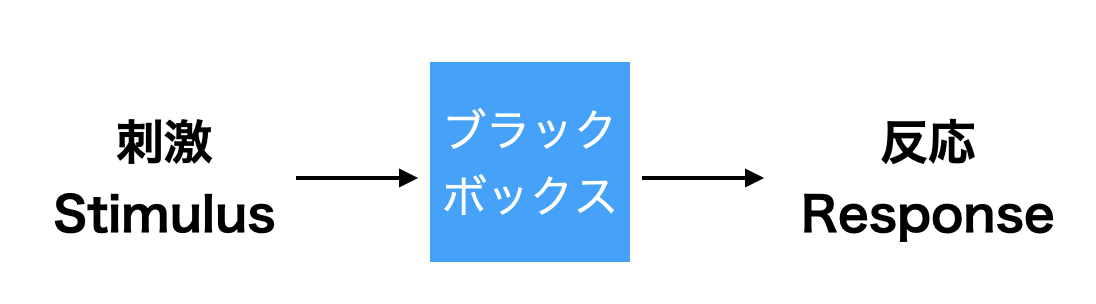
\includegraphics[keepaspectratio,width=0.65\linewidth]{figures/01_introduction/psychology_base.png}
	\caption{刺激と反応からブラックボックスを探る}
	\label{fig:01_01}
\end{figure}

心理学では科学的に考えるために，主体(人間に限らず心があると思われるのであれば何でも)に対してさまざまな刺激を与え，その反応パターンでもって「心があると言えるかも」と考えるのです。これはニュートンが「りんご$\to$?$\to$落ちる」の関係から，そこに「重力」があるのかも？ と思ったのと同じ理屈です。彼はこの関係を数式で表現したのでしたね(数学的現象主義)。「こころ」も「こうすれば$\to$心のせいで$\to$こうなる」という因果を説明する表現方法だといえます。

さきほどの図\ref{fig:01_01}もそうですが具体的な現象を抽象化して表現することで，理解が進んだり新しい解釈ができたりします。この抽象化された，理想的な状態の表現方法を\keyterm{モデル}{もでる}{model}と言います。心理学では主体に心というモデルを想定し，もしそのモデルが現実と対応しているのであれば，(理論から導かれた特定の)刺激に対して，(理論から導かれる結果としての)反応が現れるはずである，と考えることができます。そこでさまざまな刺激を考え，さまざまな反応を受け止め，心というモデルの正しさを検証しようとしているのです。

もちろん刺激にはいろいろなパターンが考えられます。それこそ無数に考えられてきました。そしてそれに対応する反応もさまざまなものがあるでしょう。1つの刺激にだって，個人差がありますから，さまざまなバリエーションのある反応が出てくるはずです。

こうしたたくさんの刺激--反応を正確に記録するために数値化が必要であり，数値化することで要約が可能になり，数式でその関係を表現することで一般化できます。その数式に実際の数値を代入することで事実に合致しているかどうかを検証できます。このように考えると，心理学で数字を使わないはずがないのです。もちろんそのほかの学問でも，数値化や数字は必須です。物理学のように純粋に数学を扱う領域もあれば，工学のように測定されたデータを扱って物理理論との対応を考える，いわゆる理系の学問では当然ですが，人文社会科学においても使わないわけはないのです。

統計は，単なる集計に関する学問ではありません。とくに「心理」統計は，心という目に見えないものを見るために，どのように測定するか，どのようにデータを取るか，と言ったところが決定的に重要です。これらは\keyterm{心理測定法}{しんりそくていほう}{psychometrics}といわれ，心理学のさまざまな領域で考えられています。しかし一度数値化されたデータが手に入れば，それからどのようにメカニズムを解釈するのか，どのようにモデルを立てていくのかについては領域を超えてさまざまな手法があります。それがこの授業，心理学データ解析でみなさんが学ぶべきことなのです。みなさんはこの後，さまざまな専門領域に進んでいきますが，得られたデータを分析するという点については共通した知識・知恵の蓄積がありますので，心理学のごく基礎的な段階から学ぶ必要があります。

数字で心がわからない，と思う人がいるかもしれませんが，これについてはどのように数字にしたのか，という心理測定の問題が理由となっているのではないでしょうか。すなわち，嬉しい気持ち，悲しい気持ちを4とか23とか言われても，そういうんじゃないんだよな，といいたくなるのはわかりますが，それは嬉しい$=4$だと誰がどうやって決めたんだ，という問題なのです。

仮に数字が正しく心の状態を表現していたとすると，その後その大量の数値から要約したり個人差を除外して，真なる状態を求めることができるかもしれません。近年はあらゆるところに人の行動が記録される機会があります。こうした記録は膨大な量に上るので，ビッグデータと呼ばれています。ビッグデータの中から，人の行動パターンを分析するのも心理統計の範疇です。

犯罪プロファイリングやマーケティングなども心理統計の応用的実践例です。もちろん臨床的介入の効果を検証するとか，実験的操作の影響力を評価することも心理統計の守備範囲です。数値化することによって，目に見えなくて触れなくてあるのかないのかもわからないものが，どの程度わからないのか，どこまでならわかるのかといったことも表現できるようになるのです。

心理学と統計法の関係，心理統計の必要性についてご理解いただけましたでしょうか。納得をいただいた上で，心理統計の具体的な話に進んでいきたいと思います。
\section{課題}
\paragraph{心理学とは何だろうか}
みなさんの中で心理学とはどういうイメージを持っていますか。この講義を受けるまえはどのように考えていましたか。この講義を受けた後で何か変わりましたか。できれば今考えている，あなたなりの心理学像を，どこかに書き起こしておくと良いでしょう。前期の終わり，あるいは一年の終わり，そして四年後にそれがどう変わるかを楽しみに。
\paragraph{心理学にどうして統計が必要なのか}
第1回は心理統計の中身に入る前に，どうして心理学なのに数字を扱って統計を学ぶのかについてを解説しました。みなさんの身近な人に，みなさんなりの言葉でこのことを説明してみてください。そのときに，心理統計と心理測定の違い，科学としての心理学，というキーワードを入れながら説明できれば完璧です\footnote{また後ほど触れることになりますが，ある人が何かを理解している，わかっているということは，そのことについてさまざまな表現を延々と生み出すことができる，ということでもあります。もし言葉に詰まったり，うまく説明できないことがあれば，そこの理解ができていないと考えられます。}。
\end{document}
